\section{Introduction}\label{S:Intro}

Advanced collision avoidance systems, lane keeping support, traffic jam assistance, and remote valet parking; they all operate on the actuators to relieve the drivers of the lateral and/or longitudinal vehicle control or make it safer for them. Well-defined tasks, such as staying in the middle of the marked lane while following the vehicle ahead, can be handled by a set-point controller \cite{handbuchFAS_Gayko2012}. And yet standard automated parking maneuvers already require a calculated trajectory\footnote{More precisely: a path, which does not have any time dependency} that must be adapted to the available parking space. As systems need to cover more and more situations, the number of degrees of freedom increase, which makes a trajectory parameterization very complex, especially when the vehicle must take numerous obstacles into account. This calls for a systematic approach based on mathematical optimization (as opposed to heuristic approaches such as potential field and elastic bands methods, see e.g. \cite{krogh1984generalized}, \cite{Brandt2008}, with their inherent limitations, cf. \cite{koren1991potential}.
In the chapter at hand, we address real-time trajectory optimization\footnote{Notice, that in control theory the term trajectory planning usually implies that there is no feedback of the actual system states on the trajectory. The dynamical system is then only stabilized by a downstream trajectory tracking controller, which is not always advisable. We therefore use the term trajectory optimization instead to be independent of the utilized stabilization concept.}, a task that an automated vehicle faces when it travels through its environment, also referred to as motion planning in robotics \cite{latombe1990robot}; \cite{lavalle2006pa}. The focus will be on methods that engage with the longitudinal and lateral vehicle movement. However, the results can be transferred to novel warning systems that can also
benefit from an optimal trajectory prediction, see e.g. \cite{eichhorn2013Maneuverprediction}. 
Speaking most generally, a trajectory optimization method is sought that can handle both structured (e.g. streets) and unstructured environments (parking lots), one that works amongst cluttered static obstacles and in moving traffic as well as exhibits a natural, human-like, anticipatory driving behavior.
Using more technical terms, the method should be easy to implement, parameterize, adapt, scale well with the number of vehicle states and the length of the optimization horizon, incorporate nonlinear, high fidelity vehicle models, combine the lateral and longitudinal motion, be complete \footnote{A complete algorithm always finds the solution if it exists.}, allow for both grid maps and object lists representations (with predicted future poses) of the obstacles, be numerically stable, and transparent in its convergence behavior (if applicable). Also, the calculation effort must be low to allow for short optimization cycles on (low performance) electronic control units so that the vehicle can quickly react to sudden changes in the environment.
Unfortunately, there is no such single method that has all these properties. And, most likely, there will never be one. However, different optimization methods can be combined to get as close as possible to the above requirements. The next section therefore gives a closer look into the basic principles of trajectory optimization and their application.

\section{Dynamic Optimization}\label{DO}

When engineers speak about optimization, they usually refer to static optimization, in which the optimization variables  $\bs{p}$  are finite, also called parameters (e.g., finding the most efficient operating point of an engine). Then optimal refers to some well-defined optimization criterion, usually the minimization of a cost function $J(\bs{p})$ (e.g., fuel consumption per hour). 
Trajectory optimization is different in that the optimization variables are functions $\bs{x}(t)$ of an independent variable $t$, usually time. It is also called dynamic or infinite-dimensional optimization. Evaluating $\bs{x}(t)$ therefore requires a cost functional (a “function of a function”), which quantifies the “quality” of the trajectory $\bs{x}(t)$ by a scalar value. 
Due to the vehicular focus, a special case will be considered, one that requires the trajectory $\bs{x}(t)$ to be consistent with some dynamical system model which has an input u. Without such model, the optimization cannot incorporate the inherent properties and physical limitations of the vehicle. This special case of dynamic optimization is called an optimal control problem (e.g., \cite{Lewis_OC}).

\subsection{Optimal Control Problem}
A fairly general formulation of the optimal control problem (OCP) reads:

Minimize the cost functional
\begin{subequations} \label{equ:optimalsteuerungsproblem}
\begin{align} \label{equ:opt_funktional}
	J(\bs{u}(t)) = \int_{t_0}^{t_f} l(\bs{x}(t),\bs{u}(t),t)\,{\rm d} t \,\,+\,\, V(\bs{x}(t_f),t_f)
\end{align}
\quad subject to the system dynamics
\begin{align} 	\label{equ:opt_systemdynamik}
	\dot{\bs{x}}(t) = \bs{f}(\bs{x}(t),\bs{u}(t),t), \quad &\bs{x}(t_0) = \bs{x}_0 
\end{align} 
\quad as well as the equality and inequality constraints
\begin{align} 	
	\bs{g}(\bs{x}(t_f),t_f) &= \bs{0}  \label{equ:zm} \\ 	
	\bs{h}(\bs{x}(t),\bs{u}(t),t) & \leq \bs{0},  \quad \forall t \in[t_0, t_f] 	\label{equ:opt_ungleichungen} \;. 
\end{align} 
\end{subequations}

In other words, for our (possibly nonlinear and time variant) system with state $\bs{x} \in \mathbb R^n$ and input $\bs{u} \in \mathbb R^m$ we seek on the interval $t\in[t_0, t_f]$ the input trajectory u(t) that minimizes the cost functional J while steering (in the truest sense of the word) the system from its initial state $x_0$ to an end state $\bs{x}(t_f)$, so that the equality and inequality constraints are fulfilled at all times. The optimal input trajectory is usually denoted by $\bs{u}^\ast(t)$ and the resulting state trajectory by $\bs{x}^\ast(t)$, 
see Fig. \ref{fig:dynamische_Optimierung_endvorgabe}. Notice that $J$ comprises integral costs $l$ and end point costs $V$ and is not only a functional of the input $\bs{u}(t)$ but also of the states $\bs{x}(t)$. Furthermore, if the final time $t_f$ is not given, it then becomes part of the optimization, so that the length of the trajectory will also be optimized.
\begin{figure}[ht]
\psfrag{1}[cr][cr][1.0]{$x_1$}
\psfrag{2}[br][br][1.0]{$x_2$}
\psfrag{x}[tc][tc][1.0]{$\bs{x}^\ast(t)$}
\psfrag{0}[cr][cr][1.0]{$\bs{x}_0$}
\psfrag{e}[tl][tl][1.0]{$t_f$}
\psfrag{o}[tl][tl][1.0]{$t_0$}
\psfrag{t}[bc][bc][1.0]{$t$}
\psfrag{g}[bc][bc][1.0]{$\bs{g}=\bs 0$}
\psfrag{h}[tc][tc][1.0]{$h\leq0$}
	\centering
  	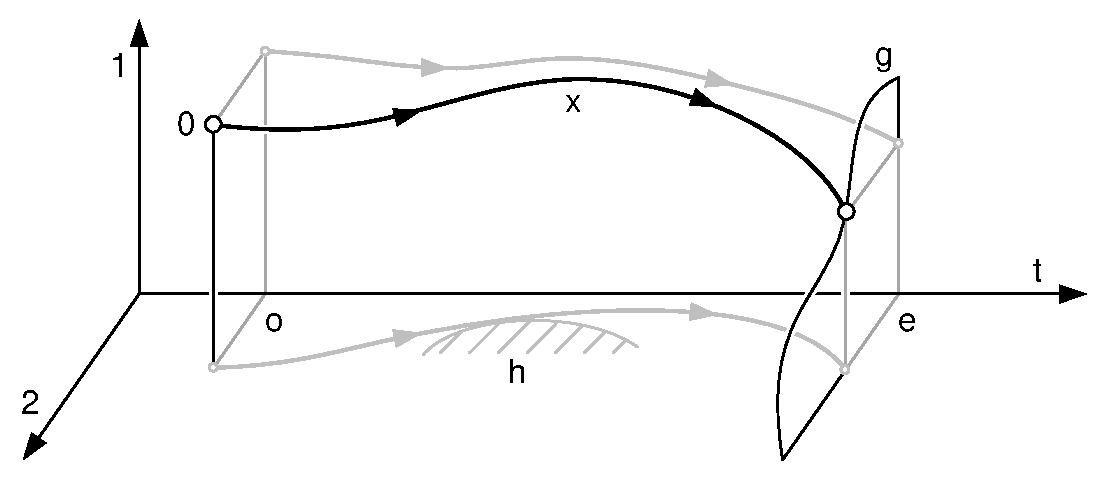
\includegraphics[width=1.\textwidth,clip, trim = 0cm 0cm 0cm 0cm]{pics/2_Darstellung_dynamische_Optimierung_endvorgabe.eps}
  	\caption[Example of an optimal trajectory]{Example of an optimal trajectory $\bs{x}^\ast (t)\in \mathbb{R}^2$ with end constraints $\bs{g}=\bs 0$ at a fixed final end time $t_f$ and inequality constraint $h\leq 0$ for $x_2$}
    \label{fig:dynamische_Optimierung_endvorgabe}
\end{figure}

\subsection{Problem Formulation for DAS and Automated Driving}
Coming back to the automotive application, equation \eqref{equ:optimalsteuerungsproblem} of the previous section describes the dynamics of the vehicle. This state space model also includes the planar motion, either relative to some reference such as the lane center, see Sect. \ref{sec:example_application_ALC}, or relative to a stationary origin, see Sect. TODO 57.3.3.4. Undesired vehicle motion such as deviations from the lane center, detours, dangerous vehicle states (e.g., large slip angles), or uncomfortable jerks, e.g., caused by hectic steering actions will be penalized in the cost functional (1). The free space prediction between the generally moving obstacles can be described by the inequality constraints (4). And the end constraints (3) can be utilized to require that the optimized vehicle trajectory will be aligned to the road at the end of the optimization interval. As will be explained in Sect. 57.5, this final state plays an important role for the stability of the “replanning” algorithm, therefore special costs 
$V(\bs{x}(t_f), t_f)$ can be introduced in (1). 

\subsection{Solving the Optimal Control Problem}
All known approaches to the OCP can be assigned to one of the following three principles, see e.g. \cite{diehl_fast_multipleshooting}.
\subsubsection{Approach I: Calculus of Variations}
The classical approach to the OCP is \textit{calculus of variations}, which delivers valuable insight in the solution. 

\textbf{Theoretical Background: Hamilton Equations}

Static optimization problems can be tackled by \textit{differential calculus}. It is well known that the first derivative of a function $J(\bs p)$  is equal to zero at a minimum (or any other stationary point). For multivariate problems we can write $\nabla\!J(\bs x) = \bs 0$
which leads to a set of (algebraic) equations that the optimum 
$\bs{p}^\ast$ must satisfy. The extension to problems with equality constraints requires the method of so-called \textit{Lagrange-multipliers}, yielding first order necessary conditions for optimality.
Analogously for dynamic optimization, variational calculus requires that the first variation of the functional $J(\bs{u}(t))$
vanishes for the optimal control function $\bs{u}^\ast$
which is often written as $\delta J(\bs{u}(t))=0$. 

In order to incorporate the system dynamics in the OCP, which constitute (differential) equality constraints, we can also apply the Lagrange-multiplier method. This yields a set of differential equations, the so-called Hamilton equations:

%x ̇=f(x,u,t)	(57.1))
%λ ̇=-∂l/∂x-[∂f/∂x]^"T"  λ	(57.2))
%0=-∂l/∂u-[∂f/∂u]^"T"  λ

\begin{subequations} \label{equ:hamiltongl}
\begin{alignat}{1}
\dot {\bs x} 				&= \bs f(\bs x, \bs u, t) \label{equ:hamilton_dgl}\\
\dot {\bs \lambda} 	&= -\frac{\partial l}{\partial \bs x} - \left[\frac{\partial \bs f}{\partial \bs x}\right]^\T \bs \lambda \label{equ:hamilton_dgl_adj}\\
\bs 0     					   &= \,\,\,\,  \frac{\partial l}{\partial \bs u} + \left[\frac{\partial \bs f}{\partial \bs u}\right]^\T \bs \lambda \label{equ:hamilton_steuergleichung}
\end{alignat}
\end{subequations}

\begin{align}
\bs x(t_0) = \bs x_0 \label{equ:fester_anfangszustand}
\end{align}



They are \textit{first order necessary conditions} for our OCP, when there are no inequality constraints (4) involved. The function $\bs \lambda(t)$
constitutes the Lagrange-multipliers, here called \textit{co-states}. Besides the initial condition
\begin{align}
\bs x(t_0) = \bs x_0 \label{equ:fester_anfangszustand}
\end{align}
the optimal trajectory must fulfill the (algebraic)\textit{ transversality conditions}, depending on whether the end state $\bs x(t_f)$
is constraint by TODO (3) and/or the final time $t_f$ is given (see e.g. \cite{Lewis_OC}). 

The simplest condition requires a fixed end state $\bs x_f$ at a given end time  $t_f$
so that
\begin{align}
\bs x(t_f) = \bs x_f \label{equ:fester_endpunkt}
\end{align}
Either way, this results in a boundary value problem, which in general needs to be solved numerically. This so-called indirect approach is very accurate but not as flexible as the direct approach that we will introduce in Sect. 57.3.2. However, for simple OCPs the resultant boundary value problem can be solved analytically, leading to fast computable optimal trajectory primitives with broad applications (see Sect. 57.4).

\subsubsection{Example Application: Automated Lane Change}\label{sec:example_application_ALC}

\subsubsection{Further Readings}


\subsubsection{Approach II: Direct Optimization Techniques}

\subsubsection{Example Application: Emergency Obstacle Avoidance}

\subsubsection{Further Readings}

\subsubsection{Approach III: Dynamic Programming}

\subsubsection{Example Application: Optimal Overtaking}

\subsubsection{Further Readings}


\section{Comparison of the Approaches}

\section{Receding Horizon Optimization}\label{S:xx}

\section{Conclusion}\label{S:yy}











